\documentclass[11pt]{article}

% load some asm stuff -
\usepackage{amssymb}
\usepackage{amsmath}
\usepackage{amsthm}
%\usepackage{palatino,lettrine}
\usepackage{fancyhdr}
\usepackage{epsfig}
\usepackage[round,comma,sort]{natbib}
\usepackage{simplemargins}
\usepackage{setspace}
\usepackage[margin=0pt,font=small,labelfont=bf]{caption}

\bibliographystyle{plos2009}

% Set the size
%\textwidth = 6.75 in
%\textheight = 9.75 in
%\oddsidemargin = 0.0 in
%\evensidemargin = 0.0 in
%\topmargin = 0.01 in
%\headheight = 0.0 in
%\headsep = 0.25 in
%\parskip = 0.15in
\doublespace

\setallmargins{1in}

\newtheorem{example}{Example}[section]
\newtheorem{thm}{Theorem}[section]
\newtheorem{property}{Property}[section]

\theoremstyle{definition}
\newtheorem{defn}[thm]{Definition}

\makeatletter
\renewcommand\subsection{\@startsection
	{subsection}{2}{0mm}
	{-0.05in}
	{-0.5\baselineskip}
	{\normalfont\normalsize\bfseries}}
\renewcommand\subsubsection{\@startsection
	{subsubsection}{2}{0mm}
	{-0.05in}
	{-0.5\baselineskip}
	{\normalfont\normalsize\itshape}}
\renewcommand\paragraph{\@startsection
	{paragraph}{2}{0mm}
	{-0.05in}
	{-0.5\baselineskip}
	{\normalfont\normalsize\itshape}}
\makeatother
\linespread{1.2}

\fancypagestyle{proposal}{\fancyhf{}%
	\fancyhead[RO,LE]{\thepage}%
	\fancyhead[LO,RE]{ChE 525 Performance of Well-Mixed Continuous and Feb-batch Cultures}%
	\renewcommand\headrulewidth{1pt}}
\pagestyle{proposal}

% Single space'd bib -
\setlength\bibsep{0pt}

\renewcommand{\rmdefault}{phv}\renewcommand{\sfdefault}{phv}

%\newboxedtheorem[boxcolor=black, background=gray!5,titlebackground=orange!20,titleboxcolor = black]{color_box_example}{Example}{test}

% Change the number format in the ref list -
\renewcommand{\bibnumfmt}[1]{#1.}

% Change Figure to Fig.
\renewcommand{\figurename}{Fig.}

%Joycelyn Chan, Joshua Lequieu, Michael Paull, Chidanand Balaji, Ryan Tasseff
%Our derivation follows closely the earlier development of Fredrickson \citep{Fredrickson:1976fk}.

% Begin ...
\begin{document}

%\begin{titlepage}
{\par\centering\textbf{\Large Performance of Well-Mixed Continuous and Feb-batch Cultures}}
\vspace{0.2in}
{\par \centering \large{Jeffrey D. Varner$^{*}$}}
\vspace{0.05in}
{\par \centering \large{School of Chemical Engineering$^{*}$}}
{\par \centering \large{Purdue University, West Lafayette IN 47907}}
\vspace{0.1in}
{\par \centering \small{Copyright \copyright\ Jeffrey Varner 2016. All Rights Reserved.}}\\

%\end{titlepage}
\date{}
\thispagestyle{empty}

\setcounter{page}{1}

\section*{Introduction}
We developed material balances for nutrients, products and cells for batch, fed-batch and continuous stirred tank bioreactors.
However, we have not considered the \textit{best} way to operate these bioreactors, for example, to maximize the amount of the product or
the rate of product production in a given time period. To explore the \textit{optimum} way to operate a bioreactor, we must specify three things;
first we need a model for the specific growth rate of cells, second we need to define a performance objective,
and last we must define any process or economic constraints the process must obey.
Let's consider each of these in turn.

\subsection*{Specific growth rate models.}
One of the most widely used models for the specific growth of simple cells on a limiting nutrient i was suggested by Monod \citep{MONOD-1949}:
\begin{equation}\label{eqn:simple-monod-single-substrate}
\mu = \mu_{g}^{max}\left(\frac{C_{i}}{K_{G,i}+C_{i}}\right)
\end{equation}where $\mu^{max}_{g}$ is the maximum specific growth rate (hr$^{-1}$), and $K_{G,i}$ is a saturation constant for nutrient i (mmol/L).
However, there have been many modifications to the Monod equation developed to describe different scenarios
such as product or nutrient \textit{inhibition}. Generally, these modifications take the form:
\begin{equation}
\mu = \mu_{g}^{max}\left(\frac{C_{i}}{K_{G,i}+C_{i}}\right)\phi\left(\mathbf{C},\mathbf{k}\right)
\end{equation}where $\mathbf{C}$ and $\mathbf{k}$ denote the concentration \textit{vector}, and a parameter vector, respectively.
For example, the inhibition of growth rate by product P could be captured by terms of the form:
\begin{equation}
\phi\left(\mathbf{C},\mathbf{k}\right) = \frac{K_{I,P}}{K_{I,P}+C_{P}}
\end{equation}or
\begin{equation}
\phi\left(\mathbf{C},\mathbf{k}\right) = 1 - \frac{\alpha C_{P}^{n}}{1 + \alpha C_{P}^{n}}
\end{equation}where $\alpha$ and $K_{I,P}$ are inhibition constants, and $n$ is called a cooperativity parameter.
Other formulations have been proposed to capture substrate inhibition. One of the most common is given by:
\begin{equation}
\mu = \mu_{g}^{max}\left(\frac{C_{i}}{K_{G,i}+C_{i} + C_{i}^{2}/K_{I,i}}\right)
\end{equation}where $K_{I,i}$ is an inhibition constant. While we'll consider only modified Monod models, there are many other models in the literature
that have been developed for particular cases. Irrespective of the model, all contain parameters that we must estimate from experimental data before we
can optimize a biological process.

\subsection*{Performance analysis of biological processes.}
The performance of a biological process can be characterized by three performance criteria, (i) the \textit{yield}, (ii) the \textit{productivity} and (iii) the \textit{titer}.
The titer is the easiest to understand, it is the concentration of the target product in the bioreactor at some endpoint time.
On the other hand, the yield and productivity describe the amount of product produced per unit of starting material consumed, and the rate of product production, respectively.

\subsubsection*{Continuous cultures.}
Before we can discuss these application of these performance metrics to continuous cultures,
we need to explore the relationship between the dilution rate and the abundance of cells in the bioreactor.
The dilution rate in a bioreactor is related to the growth rate of the organisms in the reactor through the cellmass balance.
To see this, let's split the transport terms in the cellmass balance into input and output terms:
\begin{equation}
	\sum_{s,in}^{\mathcal{S}}D_{s}X_{s} - \sum_{s,out}^{\mathcal{S}}D_{s}X_{s}+\left(\mu - k_{d}\right)X = 0
\end{equation}The input terms describe the abundance of cells being carried into the reactor by flow. In most applications we do \textit{not} have cells in any of the input streams.
This condition (known as the sterile feed assumption) reduced the cellmass balance to:
\begin{equation}
	- \sum_{s,out}^{\mathcal{S}}D_{s}X_{s}+\left(\mu - k_{d}\right)X = 0
\end{equation}Since we are assuming a well mixed bioreactor, $X_{s}\simeq{X}$ which reduces our cellmass balance to:
\begin{equation}
	\left(\mu - k_{d}\right)X - X\sum_{s,out}^{\mathcal{S}}D_{s} = 0
\end{equation}or:
\begin{equation}\label{eqn:dilution-rate-growth-rate}
	\left(\mu - k_{d}\right) = \sum_{s,out}^{\mathcal{S}}D_{s}
\end{equation}
Equation \eqref{eqn:dilution-rate-growth-rate} is an important relationship; it says that we, not the microorganism, can set how fast we want the cells to grow in the reactor.
Thus, we can \textit{externally} control the rate that \textit{intracellular} metabolites, energy (e.g., ATP) and reducing power (e.g., NADH) are used to produce new cells or products.
Of course, we can't increase the dilution rate forever as their is a maximum rate at which cells can divide. If we increase the dilution rate beyond the maximum specific growth rate, all of the cells will be carried out of the reactor and washed into downstream processing units (this is called the washout point).

We have already seen yields when we discussed batch cultures.
The yield measures the amount of product produced per unit of starting material consumed in a bioreactor. In a continuous bioreactor,
we can redefine the the apparent yield of product $i$ produced by the consumption of substrate $j$ as:
\begin{equation}\label{eqn-general-yld}
	Y_{i/j} = \left|\frac{\sum_{s}v_{s}D_{s}C_{i,s}}{\sum_{s}v_{s}D_{s}C_{j,s}}\right|
\end{equation}Equation \eqref{eqn-general-yld} is a direct measure of the ratio of actual concentrations of starting materials and products in the bioreactor.
For example, let's calculate the apparent yield of cellmass (X) on glucose (G) in a well-mixed continuous bioreactor with two sterile input streams (S1 and S2) and a single output stream (S3). Glucose is carried into the reactor in stream 1, but not stream 2. Unreacted glucose and cells are carried out the reactor in stream 3. For our reactor, the apparent yield equation becomes:
\begin{equation}
	Y_{X/G} = \left|\frac{-D_{3}C_{X,3}}{D_{1}C_{G,1} - D_{3}C_{G,3}}\right|
\end{equation}which reduces to:
\begin{equation}
	Y_{X/G} = \left|\frac{-D_{3}C_{X}}{D_{1}C_{G,1} - D_{3}C_{G}}\right|
\end{equation}after invoking the well mixed assumption.

Productivity is a measure of the rate of production or consumption of a species in a bioreactor.
For steady-state well mixed continuous bioreactors, we define the productivity as:
\begin{equation}
	\mathcal{P}_{j} = C_{j}\sum_{s,out}^{\mathcal{S}}D_{s}
\end{equation}We can also define productivity for fed-batch cultures by consider the total inflow rate.
Productivity has units of concentration per time e.g., mmol/L-hr, thus it is a measure of the rate of product production in the reactor.
Often the optimization problem for continuous cultures is to choose the dilution rate D (and/or the concentration of substrate in the feed)
such that product or cellmass productivity is maximized (Fig. \ref{fig-productivity-chemostat}).
However, this is challenging as the optimum dilution rate is very close to the washout point for the bioreactor.
Thus, while it is theoretically possible to achieve this productivity, it is practically difficult given real-world process performance.

\begin{figure*}[!ht]\centering
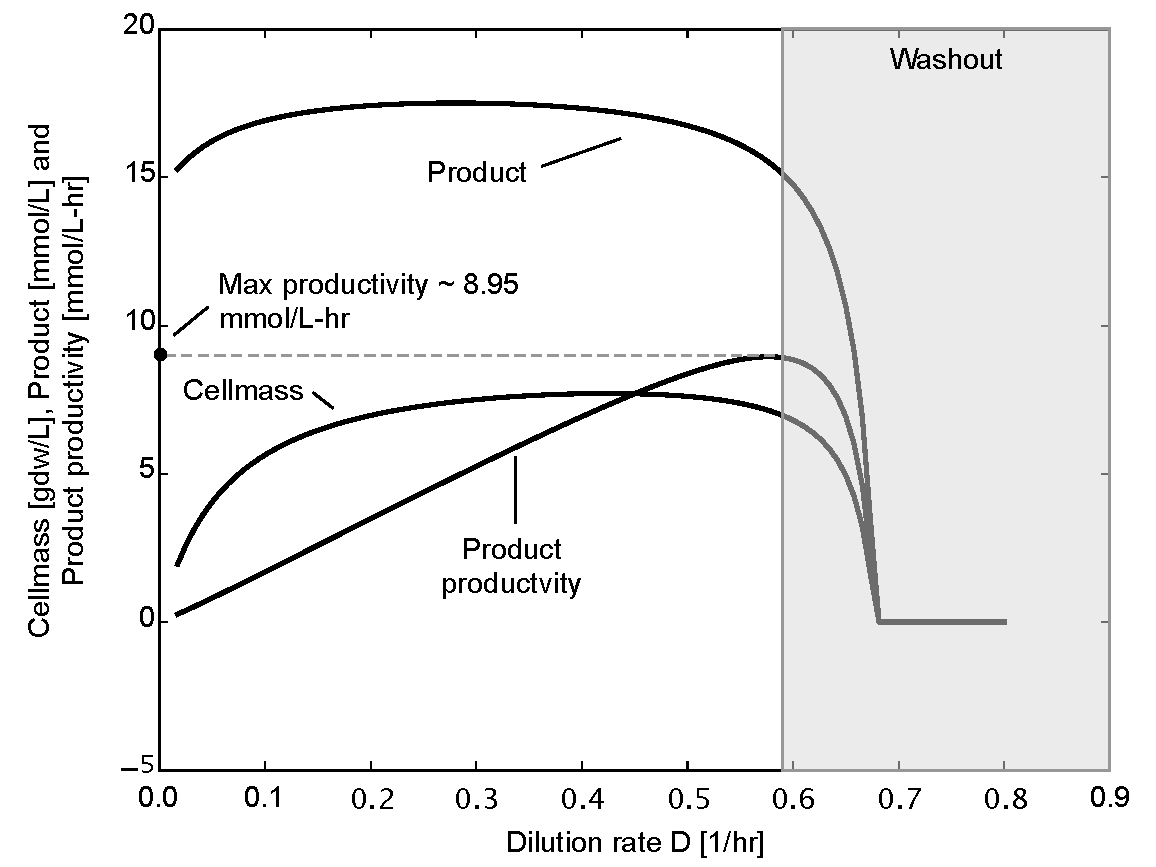
\psfig{file=figs/Productivity-Chemostat.pdf,width=0.8\textwidth}
\caption{Chemostat performance as a function of dilution rate for a typical growth associated product for well-mixed single input/output chemostat.
The x-axis denotes dilution rate D [1/hr] while the y-axis denotes the cellmass (X) [gdw/L], product (P) [mmol/L] and product productivity [mmol/L-hr].
The maximum product productivity occurs near the washout condition.}\label{fig-productivity-chemostat}
\end{figure*}


\subsubsection*{Fed-batch cultures.}
The problem of optimizing fed-batch cultures is much more difficult than a continuous culture because the bioreactor is not at a steady state.
In this case, for a given choice of \textit{design variables} (things we can change),
we must solve a dynamic system of differential equations (the species balances) and evaluate the solution $\mathbf{x}(t)$ using
our performance criteria, such as titer or productivity. For fed-batch cultures, our design variables are typically the shape of the feed ramp (the volumetric flow rate into
the bioreactor as a function of time), the starting abundance of nutrients and cells, and the length of time we run the culture. Given these design variables $\mathbf{u}$ , we will maximize the performance function $J\left(T\right)$:
\begin{equation}\label{eqn-generic-obj-function}
J\left(T\right) = \vartheta\left(\mathbf{x}\left(T\right),T\right) + \int_{t_{0}}^{T}\mathcal{L}\left(\mathbf{x},\mathbf{u},t\right)dt
\end{equation}subject the material balances, and to process or economic constraints:
\begin{eqnarray}\label{eqn-generic-constraints}
		\frac{d\mathbf{x}}{dt} &=& \mathbf{f}\left(\mathbf{x},\mathbf{u},\mathbf{\theta}\right)\\
	\mathbf{g}\left(\mathbf{x}\right)&\geq&\mathbf{0}
\end{eqnarray}
where $\vartheta\left(\mathbf{x}\left(T\right),T\right)$ and $\mathcal{L}\left(\mathbf{x},\mathbf{u},t\right)$ are specific performance functions, $\mathbf{f}\left(\mathbf{x},\mathbf{u},\mathbf{\theta}\right)$ are the material balance equations and $\mathbf{g}\left(\mathbf{x}\right)$ denote process constraints.

\begin{figure*}[!ht]\centering
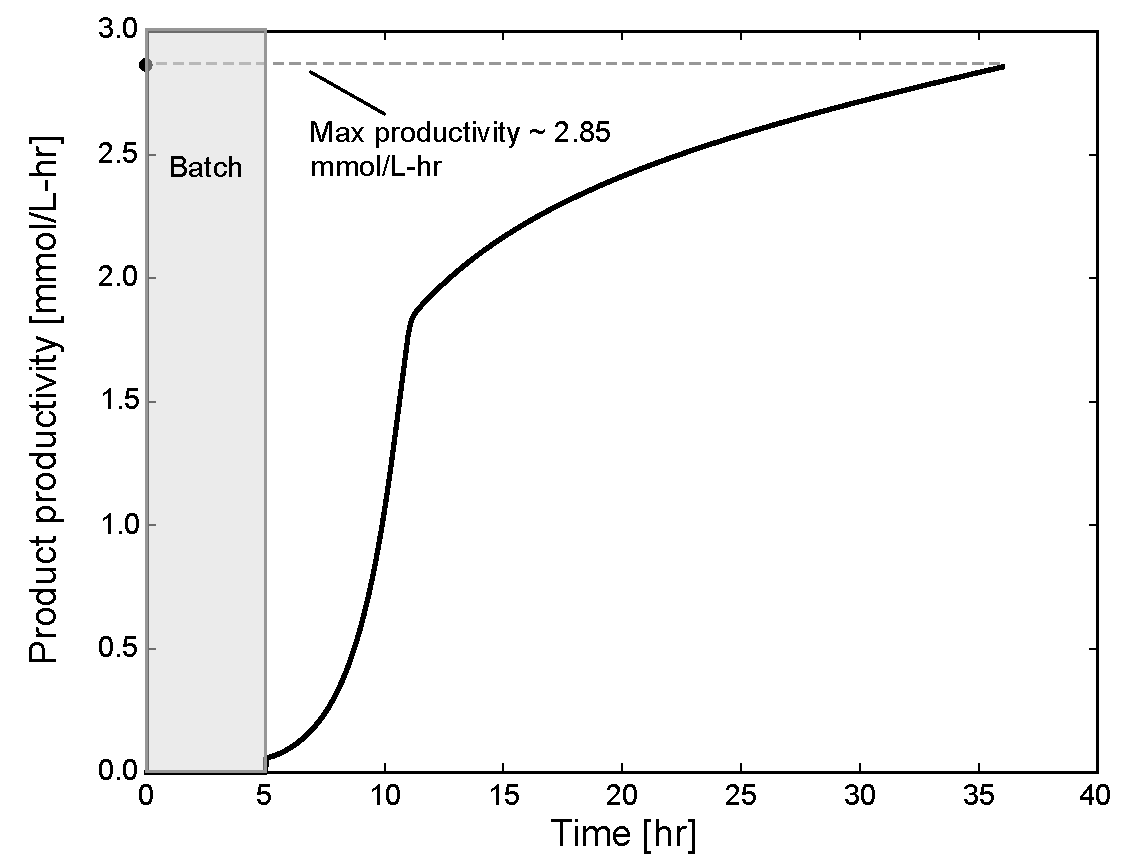
\psfig{file=figs/Productivity-Fedbatch.pdf,width=0.8\textwidth}
\caption{Fed-batch performance as a function of time for a typical growth associated product for well-mixed single input culture.
The x-axis denotes time [hr], while the y-axis denotes the product productivity [mmol/L-hr]. If operated correctly, the
fed-batch productivity increases as a function of time.}\label{fig-productivity-fedbatch}
\end{figure*}

The productivity of a fed-batch culture is \textit{less} than the equivalent chemostat culture (Fig. \eqref{fig-productivity-fedbatch}).
However, by implementing the solution of the optimization problem given by Eqn. \eqref{eqn-generic-obj-function} subject to the constraints given by Eqn. \eqref{eqn-generic-constraints},
we can increase fed-batch performance such that we asymptotically approximate chemostat performance at long times (large values of $T$).
There are many techniques to solve the fed-batch optimization problem; however, given the non-linear nature of the model equations an analytical solution is usually not possible.
In most cases, the solution must be obtained numerically using common optimization platforms such as the Optimization toolbox in MATLAB or the JuMP package in Julia \citep{julia_jump}.

\bibliography{Notes}
\end{document}
